\subsection*{7.1 Overview}
- introduce implementation environment
- introduce assumption
\noindent To implement a prototype of the proposed framework, we used the Ethereum smart contract and Ganache Testnet implementation. We created the smart contracts by Solidity and configured Ganache as an Ethereum network environmnet. It ran under Solidity compiler version 0.4.24 with Ganache 1.1.0. We also leveraged Truffle, a popular framework in Ethereum with the version v4.1.14, and web3.js 1.0.0-beta.35, a collection of modules which contain specific functionality for the ethereum ecosystem. Currently, the AAA provides service as an JavaScript file, which is run under Node.js v10.2.1 bundled with node-localStorage package for storing general policies and verification key-pairs.

Specific AAA implementation is presented in \autoref{fig:imple}.
\begin{figure}[h!]
  \centering
  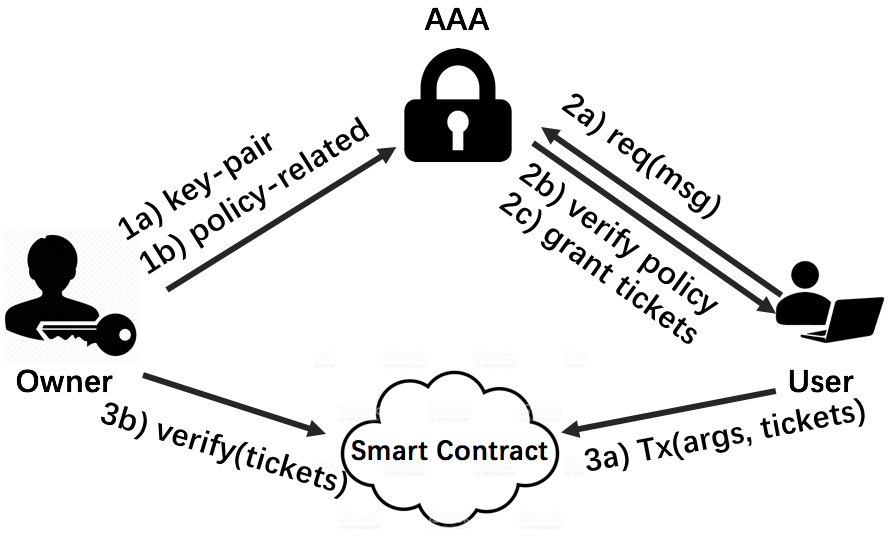
\includegraphics[width=1.0\linewidth]{fig/imple}
  \caption{Specific AAA implementation.}
  \label{fig:imple}
\end{figure}

\subsection*{7.2 Details}
- introduce each entities 

\subsection*{7.3 Evaluation}
- introduce overhead
- storage cost
- gas cost
- build model(if applicable)


